% !TEX root=../MA119-Main.tex

\paragraph*{Logarithmic Function}
	For $x>0$, $b>0$ and $b\neq 1$, there is a unique number $y$ satisfying the equation $b^y=x$. We denote the unique number $y$ by $\log_bx$, read as logarithm to the base $b$ of $x$.  In other words, the defining relation between exponentiation and logarithm is
	\[ y=\log_bx \quad\text{if and only if} \quad b^y=x.\]
	The function $f(x)=\log_bx$ is called the logarithmic function $f$ of $x$ with the base $b$.

	Graphs of logarithmic functions:
	\begin{multicols}{2}
		\begin{center}
			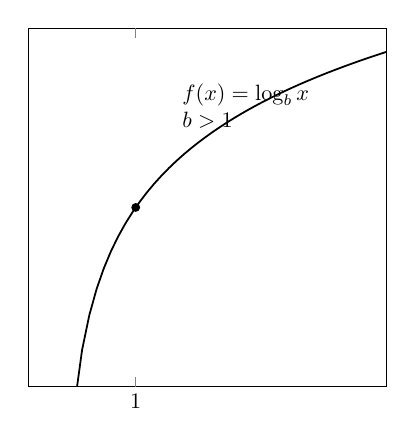
\begin{tikzpicture}[scale=0.8]
				\begin{axis}[%grid=both,
						unit vector ratio=1 1,
						xmin=-0.5,
						xmax=4.5,
						ymax=2.5,
						ymin=-2.5,
						xtick=\empty,ytick=\empty,
						extra x ticks={1},
						%  axis lines = middle,xlabel=$x$,ylabel=$y$,
						% x label style={anchor=west}, y label style={anchor=south},
						% %label style ={at={(ticklabel cs:1.1)}, font={\tiny}}
					]
					\addplot[thick, samples=100, y domain=-2.5:2.5]   {ln(x)/ln(2)};
					% \addplot[thick, samples=100, y domain=-2.5:2.5]   {-ln(x)/ln(2)};
					% \node[anchor=north] at (axis cs:2.75,-1)   {\parbox{2.5cm}{$f(x)=\log_b x$\\ $0< b<1$}};
					\node[anchor=south] at (axis cs:2.75,1)   {\parbox{2.5cm}{$f(x)=\log_bx$\\ $b>1$}};
					\node[circle,fill=black,inner sep=0pt,minimum size=4pt] at (1,0) {};
				\end{axis}
			\end{tikzpicture}
		\end{center}

		\columnbreak

		\begin{center}
			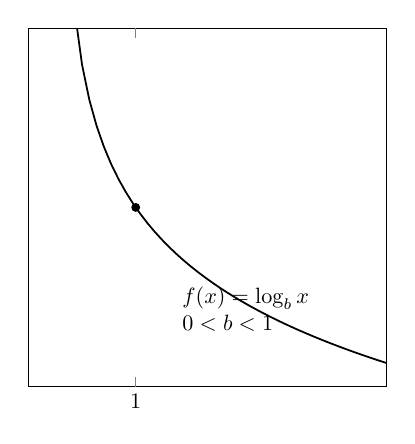
\begin{tikzpicture}[scale=0.8]
				\begin{axis}[%grid=both,
						unit vector ratio=1 1,
						xmin=-0.5,
						xmax=4.5,
						ymax=2.5,
						ymin=-2.5,
						xtick=\empty,ytick=\empty,
						extra x ticks={1},
						%  axis lines = middle,xlabel=$x$,ylabel=$y$,
						% x label style={anchor=west}, y label style={anchor=south},
						% %label style ={at={(ticklabel cs:1.1)}, font={\tiny}}
					]
					% \addplot[thick, samples=100, y domain=-2.5:2.5]   {ln(x)/ln(2)};
					\addplot[thick, samples=100, y domain=-2.5:2.5]   {-ln(x)/ln(2)};
					\node[anchor=north] at (axis cs:2.75,-1)   {\parbox{2.5cm}{$f(x)=\log_b x$\\ $0< b<1$}};
					% \node[anchor=south] at (axis cs:2.75,1)   {\parbox{2.5cm}{$f(x)=\log_bx$\\ $b>1$}};
					\node[circle,fill=black,inner sep=0pt,minimum size=4pt] at (1,0) {};
				\end{axis}
			\end{tikzpicture}
		\end{center}
	\end{multicols}

\paragraph*{Common Logarithms and Natural Logarithms}
	A logarithmic function $f(x)$ with base 10 is called the common logarithmic function and denoted by $f(x)=\log x$.

	A logarithmic function $f(x)$ with base the natural number $e$ is called the natural logarithmic function and denoted by $f(x)=\ln x$.

	\paragraph*{Basic Properties of Logarithms}
	When $b>0$ and $b\neq 1$, and $x>0$, we have
	\begin{enumerate}
		\item $b^{\log_bx}=x$.
		\item $\log_b(b^x)=x$.
		\item $\log_bb=1$ and $\log_b1=0$.
	\end{enumerate}

	\begin{example}
		Convert between exponential and logarithmic forms.\\
		\begin{enumerate*}[label={(\arabic*)~}]
			\item $\log x=\frac{1}{2}$
			\item $3^{2x-1}=5$\hfill\null
		\end{enumerate*}
	\end{example}
	\begin{solution} When converting between exponential and logarithmic forms, we move the base from one side to the other side, then add or drop the log sign.
		\begin{enumerate}[label={(\arabic*)~}]
			\item Move the base 10 to the right side and drop the log from the left:\\
			      \centerline{$x=10^{\frac{1}{2}}$.}
			\item Move the 3 to the right and add log the the right:\\
			      \centerline{$2x-1=\log_35$.}
		\end{enumerate}
	\end{solution}


	\begin{example}
		Evaluate the logarithms.\\
		\begin{enumerate*}[label={(\arabic*)~}]
			\item $\log_42$
			\item $10^{\log(\frac{1}{2})}$
			\item $\log_5(e^0)$
			\hfill\null
		\end{enumerate*}
	\end{example}
	\begin{solution}The key is to rewrite the log and the power so that they have the same base.
		\begin{enumerate}[label=\emph{(\arabic*)~}]
			\item $\log_42= \log_44^{\frac{1}{2}}=\frac{1}{2}$.
			\item $10^{\log\frac{1}{2}}=10^{\log_{10}\frac{1}{2}}=\frac12$
			\item $\log_5(e^0)=\log_51=0$
			      \hfill\null
		\end{enumerate}
	\end{solution}


	\begin{example}
		Find the domain of the function $f(x)=\ln(2-3x)$.
	\end{example}
	\begin{solution}
		The function has a real output if $2-3x>0$. Solving the inequality, we get $x<\frac{2}{3}$. So the domain of the function is $(-\infty, \frac{2}{3})$.
	\end{solution}


\newpage

\begin{exercise}
	Write each equation into equivalent exponential form.

	\noindent
	\begin{enumerate*}[label={(\arabic*)~}]
		\item  $\log_37=y$
		\item  $3=\log_b64$ 
		\item $\log x=y$
		\item $\ln(x-1)=c$
		\hfill\null
	\end{enumerate*}
\end{exercise}

%%%%%%
\vfill
\begin{center} \hfill
	\raisebox{0.5em}{
		\rotatebox{\rotationdegree}{
			\parbox{\textwidth}{
				\begin{enumerate*}[label={\theexer~(\arabic*)~}]
					\item $3^y=7$
					\item $b^3=64$
					\item $x=10^y$
					\item $x-1=e^c$
					\hfill\null
				\end{enumerate*}
			}
		}
	}
\end{center}

\begin{exercise}
	Write each equation into equivalent logarithmic form.

	\noindent
	\begin{enumerate*}[label={(\arabic*)~}]
		\item  $7^x=10$
		\item  $b^5=2$
		\item $e^{2y-1}=x$
		\item $10^x=c^2+1$
		\hfill\null
	\end{enumerate*}
\end{exercise}

%%%%%%
\vfill
\begin{center} \hfill
	\raisebox{0.5em}{
		\rotatebox{\rotationdegree}{
			\parbox{\textwidth}{
				\begin{enumerate*}[label={\theexer~(\arabic*)~}]
					\item $x=\log_710$
					\item $\log_b2=5$
					\item $2y-1=\ln x$
					\item $x=\log(c^2+1)$
					\hfill\null
				\end{enumerate*}
			}
		}
	}
\end{center}


\begin{exercise}
	Evaluate.\\
	\noindent
	\begin{enumerate*}[label={(\arabic*)~}]
		\item \parbox{0.2\textwidth}{ $\log_216$ }
		\item \parbox{0.2\textwidth}{ $\log_93$ }
		\item \parbox{0.2\textwidth}{ $\log 10$ }
		\item \parbox{0.2\textwidth}{ $\ln 1$ }
		\hfill\null
	\end{enumerate*}
\end{exercise}

%%%%%%
\vfill
\begin{center} \hfill
	\raisebox{0.4em}{
		\rotatebox{\rotationdegree}{
			\parbox{\textwidth}{
				\begin{enumerate*}[label={\theexer~(\arabic*)~}]
					\item $4$
					\item $\frac12$
					\item $1$
					\item $0$
					\hfill\null
				\end{enumerate*}
			}
		}
	}
\end{center}


\newpage

\begin{exercise}
	Evaluate.\\
	\noindent
	\begin{enumerate*}[label={(\arabic*)~}]
		\item \parbox{0.2\textwidth}{$e^{\ln 2}$ }
		\item \parbox{0.2\textwidth}{$\log 10^{\frac13}$ }
		\item \parbox{0.2\textwidth}{ $\ln(\sqrt{e})$ }
		\item \parbox{0.2\textwidth}{$\log_2(\frac12)$ }
		\hfill\null
	\end{enumerate*}
\end{exercise}

%%%%%%
\vfill
\begin{center} \hfill
	\raisebox{0.4em}{
		\rotatebox{\rotationdegree}{
			\parbox{\textwidth}{
				\begin{enumerate*}[label={\theexer~(\arabic*)~}]
					\item $2$
					\item $\frac13$
					\item $\frac12$
					\item $-1$
					\hfill\null
				\end{enumerate*}
			}
		}
	}
\end{center}


\begin{exercise}Find the domain of the function $f(x)=\log(x-5)$. Write in interval notation.
\end{exercise}
%%%%%%
\vfill
\begin{center} \hfill
	\raisebox{0.4em}{
		\rotatebox{\rotationdegree}{
			\parbox{\textwidth}{
				\begin{enumerate*}[label={\theexer~}]
					\item	$(5,+\infty)$ \hfill\null
				\end{enumerate*}
			}
		}
	}
\end{center}

\begin{exercise}
	Sketch the graph of each function and find its range.\\
	\noindent
	\begin{enumerate*}[label=(\arabic*)~]
		\item $f(x)=\log_2x$
		\item $f(x)=\log_{\frac12} x$\hfill\null
	\end{enumerate*}

	\noindent
	\begin{minipage}{\textwidth}
		\begin{minipage}{0.5\textwidth}
			\begin{center}
				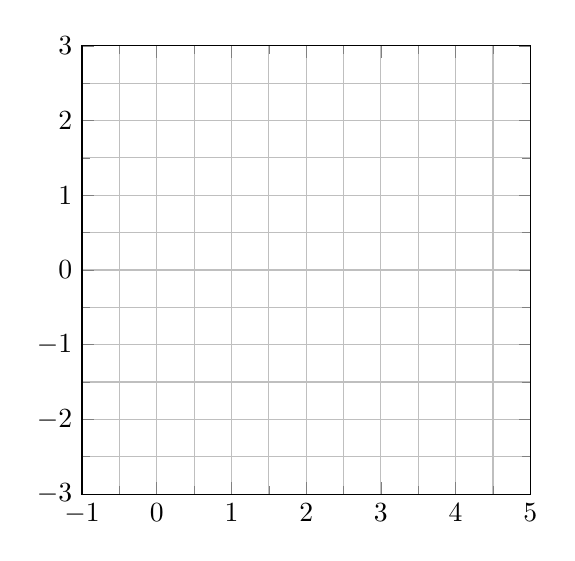
\begin{tikzpicture}
					\begin{axis}[
							grid=both,
							unit vector ratio*=1 1,
							xmin=-1,
							xmax=5,
							ymax=3,
							ymin=-3,
							ytick={-3,-2,...,3},
							xtick={-1,0,...,5},
							minor tick num=1,
							%  axis lines = middle,xlabel=$x$,ylabel=$y$,
							% x tick label style={yshift=0.5ex,font={\tiny}}, y tick label style={xshift=0.5ex, font={\tiny}}, label style ={at={(ticklabel cs:1.1)}, font={\tiny}}
						]
						%\addplot[thick, samples=100,domain=1:3.82, name path=A, -stealth]   {(x-2)^2+1};
						% \addplot[thick, draw] (1, 2)--(-1.95,1.5);
						% \node[draw,shape=circle, minimum size=1.25mm,inner sep=0pt,outer sep=0pt] at (-2,1.5) {};
					\end{axis}
				\end{tikzpicture}
			\end{center}
		\end{minipage}
		\begin{minipage}{0.5\textwidth}

			\begin{center}
				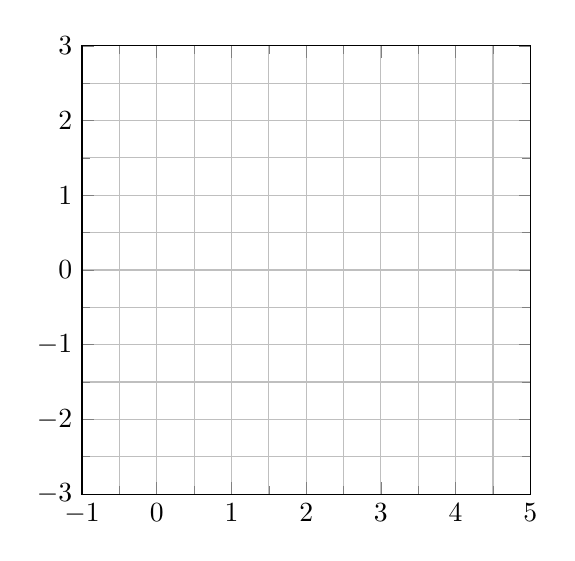
\begin{tikzpicture}
					\begin{axis}[
							grid=both,
							unit vector ratio*=1 1,
							xmin=-1,
							xmax=5,
							ymax=3,
							ymin=-3,
							ytick={-3,-2,...,3},
							xtick={-1,0,...,5},
							minor tick num=1,
						]
						%\addplot[thick, samples=100,domain=1:3.82, name path=A, -stealth]   {(x-2)^2+1};
						% \addplot[thick, draw] (1, 2)--(-1.95,1.5);
						% \node[draw,shape=circle, minimum size=1.25mm,inner sep=0pt,outer sep=0pt] at (-2,1.5) {};
					\end{axis}
				\end{tikzpicture}
			\end{center}
		\end{minipage}
	\end{minipage}
\end{exercise}
\vspace*{\stretch{0.5}}

